\documentclass[../main.tex]{subfiles}
\begin{document}


\subsection{Data Model}
In our draft implementation of the data as fiber bundle model, we represent $K$ as a simplacial complex. 

\begin{figure}[ht]
    \label{fig:simplex}
    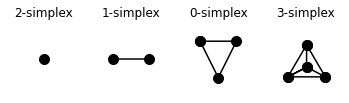
\includegraphics{figures/sections/math/simplex.png}
    \caption{Simplices encode the connectivity of the data, from fully disconnected (0 simplex) observations to all observations are connected to at least 3 other observations. Higher order simplicies are outside the scope of this paper.}
\end{figure}

%% k is a triangularizable topological space 
One way to represent the topological space K is as a set composed of simplices, such as those shown in figure~\ref{fig:simplex}. Simplices are a way of encoding the connectivity of each observation ($\sigma(k)$) to another: %%formula for simplacial complexes/simplacial sets

% replace this table w/ a diagram that shows this 
\begin{description}
    \item[0-simplex] discrete observations (inventory records)
    \item[1-simplex] 1D continuos data (timeseries)
    \item[2-simplex] 2D continuos data (map)
    \item[3-simplex] 3D continuos data (video)
\end{description}
\end{document}